%# -*- coding:utf-8 -*-
\begin{apdix}
\appendix
% \counterwithout{section}{chapter}
\setcounter{chapter}{1}
% \section{\reftheorem{thm:UVcvx}的证明}\label{sec:thmproof}
% \esection{Proof of \refetheorem{thm:UVcvx}}
%     \begin{theorem}\label{theorem:thm0}\kaishu
%         $\norm{(\mydiag(\mathbfcal{X}\times_{1}\boldsymbol{U}\times_{2}\boldsymbol{V}))^{\top} - \boldsymbol{F}}_{F}^{2}$分别对$\boldsymbol{U}$或$\boldsymbol{V}$都是凸的。
%     \end{theorem}
    
%     \begin{proof}
%         我们首先证明$\norm{(\mydiag(\mathbfcal{X}\times_{1}\boldsymbol{U}\times_{2}\boldsymbol{V}))^{\top} - \boldsymbol{F}}_{F}^{2}$对矩阵$\boldsymbol{U}$的每一行$\boldsymbol{u}_{i:}$都是凸的。简单的计算表明
%         \begin{equation*}
%             \nabla_{\boldsymbol{u}_{i:}}^{2}\left(\norm{\left(\mydiag\left(\mathbfcal{X}\times_{1}\boldsymbol{U}\times_{2}\boldsymbol{V}\right)\right)^{\top} - \boldsymbol{F}}_{F}^{2}\right) = 2\sum_{k=1}^{n}\boldsymbol{X}^{(k)}\boldsymbol{v}_{i:}^{\top}\boldsymbol{v}_{i:}{\boldsymbol{X}^{(k)}}^{\top}\succeq 0.
%         \end{equation*}
%         因此,我们可以得出以下结论:$\norm{(\mydiag(\mathbfcal{X}\times_{1}\boldsymbol{U}\times_{2}\boldsymbol{V}))^{\top} - \boldsymbol{F}}_{F}^{2}$对矩阵$\boldsymbol{U}$的每一行$\boldsymbol{u}_{i:}$都是凸的。同样地,我们也可以类似地证明$\norm{(\mydiag(\mathbfcal{X}\times_{1}\boldsymbol{U}\times_{2}\boldsymbol{V}))^{\top} - \boldsymbol{F}}_{F}^{2}$对矩阵$\boldsymbol{V}$的每一行$\boldsymbol{v}_{i:}$也都是凸的。我们在此处省略证明,以防赘述。
%     \end{proof}
    
%     \begin{theorem}\kaishu
%         $\norm{(\mydiag(\mathbfcal{X}\times_{1}\boldsymbol{U}\times_{2}\boldsymbol{V}))^{\top} - \boldsymbol{F}}_{F}^{2}$分别对$\boldsymbol{U}$或$\boldsymbol{V}$都是凸的。
%     \end{theorem}
    
%     \begin{proof}
%         这是由于我们有
%         \begin{equation*}
%         \begin{aligned}
%             &\norm{\left(\mydiag\left(\mathbfcal{X}\times_{1}\left(\lambda\boldsymbol{Z}_{1}+\left(1-\lambda\right)\boldsymbol{Z}_{2}\right)\times_{2}\boldsymbol{V}\right)\right)^{\top} - \boldsymbol{F}}_{F}^{2} \\=& \sum_{i=1}^{c}\norm{\left(\mydiag\left(\mathbfcal{X}\times_{1}\left(\lambda(\boldsymbol{z}_{1})_{i:}+\left(1-\lambda\right)(\boldsymbol{z}_{2})_{i:}\right)\times_{2}\boldsymbol{v}_{i:}\right)\right)^{\top} - \boldsymbol{f}_{i}}_{F}^{2} \\\leq& \sum_{i=1}^{c}\left(\lambda\norm{\left(\mydiag\left(\mathbfcal{X}\times_{1}(\boldsymbol{z}_{1})_{i:}\times_{2}\boldsymbol{v}_{i:}\right)\right)^{\top} - \boldsymbol{f}_{i}}_{F}^{2} + \left(1-\lambda\right)\norm{\left(\mydiag\left(\mathbfcal{X}\times_{1}(\boldsymbol{z}_{2})_{i:}\times_{2}\boldsymbol{v}_{i:}\right)\right)^{\top} - \boldsymbol{f}_{i}}_{F}^{2}\right)\\=& \lambda\norm{\left(\mydiag\left(\mathbfcal{X}\times_{1}\boldsymbol{Z}_{1}\times_{2}\boldsymbol{V}\right)\right)^{\top} - \boldsymbol{F}}_{F}^{2} + \left(1-\lambda\right)\norm{\left(\mydiag\left(\mathbfcal{X}\times_{1}\boldsymbol{Z}_{2}\times_{2}\boldsymbol{V}\right)\right)^{\top} - \boldsymbol{F}}_{F}^{2},
%         \end{aligned}
%         \end{equation*}
%         其中不等号部分使用了\reftheorem{theorem:thm0}。依据凸函数的定义\ucite{boyd2004convex},$\boldsymbol{U}$部分的证明就完成了。同样的证明方法也可应用在$\boldsymbol{V}$上。为了避免冗余,我们不再赘述。
%     \end{proof}
    
%     \begin{lemma}\kaishu
%         $\norm{\boldsymbol{X}}_{2,1}$关于$\boldsymbol{X}$是一个凸函数。
%     \end{lemma}
    
%     \begin{proof}
%         我们首先证明$\ell_{2,1}$范数的确是一种范数。简单的计算表明
%         \begin{itemize}
%             \item $\norm{\boldsymbol{0}}_{2,1}=0$,
%             \item 若$\boldsymbol{X}\in\mathbb{R}^{m\times n}$,则$\norm{\alpha\boldsymbol{X}}_{2,1}=\sum_{j=1}^{m}\norm{\alpha\boldsymbol{x}_{j:}}_{2}=\alpha\sum_{j=1}^{m}\norm{\boldsymbol{x}_{j:}}_{2}=\alpha\norm{\boldsymbol{X}}_{2,1}$,
%             \item 若$\boldsymbol{X}\in\mathbb{R}^{m\times n},\boldsymbol{Y}\in\mathbb{R}^{m\times n}$,则$\norm{\boldsymbol{X}+\boldsymbol{Y}}_{2,1}=\sum_{j=1}^{m}\norm{\boldsymbol{x}_{j:}+\boldsymbol{y}_{j:}}_{2}\leq\sum_{j=1}^{m}\norm{\boldsymbol{x}_{j:}}_{2}+\sum_{j=1}^{m}\norm{\boldsymbol{y}_{j:}}_{2}=\norm{\boldsymbol{X}}_{2,1}+\norm{\boldsymbol{Y}}_{2,1}$,其中不等式部分使用了$\ell_{2}$范数的性质。
%         \end{itemize}
%         因此,$\ell_{2,1}$的确是一种范数。由于所有的范数都是凸的\ucite{boyd2004convex},我们的定理即证。
%     \end{proof}
    
%     \begin{theorem}\kaishu
%         $\norm{\boldsymbol{U}^{\top}\odot\boldsymbol{V}^{\top}}_{2,1}$分别对$\boldsymbol{U}$或$\boldsymbol{V}$都是凸的。
%     \end{theorem}
    
%     \begin{proof}
%         由于
%         \begin{equation*}
%             \operatorname{vec}\left(\boldsymbol{U}^{\top} \odot \boldsymbol{V}^{\top}\right)=\left(\boldsymbol{I}_{n_{1}c} \odot\left(\boldsymbol{V}^{\top}\left(\boldsymbol{I}_{c} \otimes \boldsymbol{1}^{\top}_{n_{1}}\right)\right)\right)\operatorname{vec}\left(\boldsymbol{U}^{\top}\right),
%         \end{equation*}
%         因此,$\boldsymbol{U}\mapsto\boldsymbol{U}^{\top}\odot\boldsymbol{V}^{\top}$可以看作是$\boldsymbol{U}$的一个线性函数。同样地,我们也可以推出,$\boldsymbol{U}^{\top}\odot\boldsymbol{V}^{\top}$也是$\boldsymbol{V}$的一个线性函数。由于凸函数与线性函数的复合函数仍然是凸函数\ucite{boyd2004convex},那我们就得到了我们想要的结论。
%     \end{proof}
    
%     \begin{corollary}
%         $\alpha\norm{(\mydiag(\mathbfcal{X}\times_{1}\boldsymbol{U}\times_{2}\boldsymbol{V}))^{\top} - \boldsymbol{F}}_{F}^{2} + \beta \norm{\boldsymbol{U}^{\top}\odot\boldsymbol{V}^{\top}}_{2,1}$对$\boldsymbol{U}$或$\boldsymbol{V}$分别是凸的。
%     \end{corollary}
    
%     \begin{proof}
%         由于凸函数的非负线性组合仍然还是凸函数\ucite{boyd2004convex},那么我们就得到了我们想要的结论。
%     \end{proof}
    
% \section{非负矩阵分解的Lee-Seung算法及其下降性}\label{sec:nmf-dec}
% \esection{The Lee-Seung Algorithm for Nonnegative Matrix Factorization and Its Decreasability}
% 在这一小节,我们介绍用于优化非负矩阵分解的目标函数的Lee-Seung算法,介绍它的下降性。
% \subsection{非负矩阵分解的典范形式}
% \esubsection{The Canonical Form of Nonnegative Matrix Factorization}
% 给定一个矩阵$\boldsymbol{V}\in\mathbb{R}^{n\times m}$,非负矩阵分解即如下数学优化模型
% \begin{equation*}
%     \begin{aligned}
%     & \underset{\smash[b]{\substack{\boldsymbol{W},\boldsymbol{H}}}}{\min}
%     & &  \norm{\boldsymbol{V}-\boldsymbol{W}\boldsymbol{H}}_{F}^{2}\\
%     & \text{s.t.}
%     & & \boldsymbol{W},~\boldsymbol{H}\geq 0,
%     \end{aligned}
% \end{equation*}
% 其中$\boldsymbol{W}\in\mathbb{R}^{n\times r}$,$\boldsymbol{H}\in\mathbb{R}^{r\times m}$。

% \subsection{Lee-Seung算法}
% \esubsection{The Lee-Seung Algorithm}
% 用于优化非负矩阵分解的经典Lee-Seung算法即反复用如下乘法更新公式迭代更新参数矩阵$\boldsymbol{W}$和$\boldsymbol{H}$。
% \begin{equation*}
% \begin{aligned}
%     \boldsymbol{W}\leftarrow\boldsymbol{W}\oast\left(\frac{\boldsymbol{V}\boldsymbol{H}^{\top}}{\boldsymbol{W}\boldsymbol{H}\boldsymbol{H}^{\top}}\right),~\boldsymbol{H}\leftarrow\boldsymbol{H}\oast\left(\frac{\boldsymbol{W}^{\top}\boldsymbol{V}}{\boldsymbol{W}^{\top}\boldsymbol{W}\boldsymbol{H}}\right).
% \end{aligned}
% \end{equation*}

% 我们把Lee-Seung算法总结至\refalg{alg:leeseung}中。

% \begin{algorithm}[t]
% 	\begin{algorithmic}[1]
% 	\REQUIRE 矩阵$\boldsymbol{V}$。
% 	\ENSURE 优化完毕后的参数矩阵$\boldsymbol{W}$和$\boldsymbol{H}$。
% 	\STATE $k\leftarrow 1$,并随机初始化$\boldsymbol{W}$和$\boldsymbol{H}$;
% 	\WHILE{$k<\Phi$并且算法未收敛}
%     \STATE $\boldsymbol{W}\leftarrow\boldsymbol{W}\oast(({\boldsymbol{V}\boldsymbol{H}^{\top}})\oslash({\boldsymbol{W}\boldsymbol{H}\boldsymbol{H}^{\top}}))$;
%     \STATE $\boldsymbol{H}\leftarrow\boldsymbol{H}\oast(({\boldsymbol{W}^{\top}\boldsymbol{V}})\oslash({\boldsymbol{W}^{\top}\boldsymbol{W}\boldsymbol{H}}))$;
% 	\STATE $k\leftarrow k+1$
% 	\ENDWHILE
% 	\RETURN $\boldsymbol{W}_{k}$以及$\boldsymbol{H}_{k}$;
% 	\end{algorithmic}
% 	\captionsetup{labelsep=period,font=bf}
% 	\caption{Lee-Seung算法}
% 	\label{alg:leeseung}
% \end{algorithm}

% 此外,文献\ucite{lee2001algorithms}还给出了如下关于Lee-Seung算法的下降性定理。

% \begin{lemma}[\ucite{lee2001algorithms}]\label{lemma:lee-desc}\kaishu
%     基于\refalg{alg:leeseung},典范型非负矩阵分解的目标函数$\norm{\boldsymbol{V}-\boldsymbol{W}\boldsymbol{H}}_{F}^{2}$在\refalg{alg:leeseung}的每一步都会得到下降。
% \end{lemma}

% \subsection{Lee-Seung算法的下降性}
% \esubsection{The Decreasability of the Lee-Seung Algorithm}
% 在本小节,我们证明Lee-Seung算法的下降性\footnote{对于Lee-Seung算法收敛性更全面的讨论与证明,我们推荐读者阅读文献\ucite{lin2007convergence}。}。我们首先需要下面几个定义来辅助说明主要的引理。

% \begin{definition}[辅助函数\ucite{lee2001algorithms}]\kaishu
%     若一个函数$\Gamma(\boldsymbol{X},\underline{\boldsymbol{X}})$同时对可行域内所有的$\boldsymbol{X}$和$\underline{\boldsymbol{X}}$满足$\Gamma(\boldsymbol{X},\underline{\boldsymbol{X}})\geq\Psi(\boldsymbol{X})$且$\Gamma(\boldsymbol{X},\boldsymbol{X})=\Psi(\boldsymbol{X})$,那我们说$\Gamma(\boldsymbol{X},\underline{\boldsymbol{X}})$是$\Psi(\boldsymbol{X})$的一个辅助函数。
% \end{definition}
    
% \begin{lemma}[辅助函数的下降性\ucite{lee2001algorithms}]\label{lemma:aux_ppt}\kaishu
% 若$\Gamma(\boldsymbol{X},\underline{\boldsymbol{X}})$为$\Psi(\boldsymbol{X})$的一个辅助函数,则基于更新公式$\boldsymbol{X}_{t+1}=\arg\min_{\boldsymbol{X}}\Gamma(\boldsymbol{X},\boldsymbol{X}_{t})$,$\Psi(\boldsymbol{X})$在每一步都是下降的。
% \end{lemma}
% \begin{proof}
% 这是由于$\Psi(\boldsymbol{X}_{t+1})\leq\Gamma(\boldsymbol{X}_{t+1},\boldsymbol{X}_{t})\leq\Gamma(\boldsymbol{X}_{t},\boldsymbol{X}_{t})=\Psi(\boldsymbol{X}_{t})$.
% \end{proof}

% \begin{lemma}[NMF目标函数的一个辅助函数\ucite{lee2001algorithms}]\kaishu
%     记$\Psi(\boldsymbol{h}_{:i})=(1/2)\norm{\boldsymbol{v}_{:i}-\boldsymbol{W}\boldsymbol{h}_{:i}}_{2}^{2}$。则函数
%     \begin{equation*}
%     \begin{aligned}
%         \Gamma(\boldsymbol{h}_{:i},\underline{\boldsymbol{h}}_{:i})=&\Psi(\underline{\boldsymbol{h}}_{:i})+\left(\boldsymbol{h}_{:i}-\underline{\boldsymbol{h}}_{:i}\right)^{\top}\nabla\Psi(\underline{\boldsymbol{h}}_{:i})\\&+\frac{1}{2}\left(\boldsymbol{h}_{:i}-\underline{\boldsymbol{h}}_{:i}\right)^{\top}
%         \begin{pmatrix}
%             \frac{\left(\boldsymbol{w}_{:1}^{\top}\boldsymbol{W}\underline{\boldsymbol{h}}_{:i}\right)}{\underline{\boldsymbol{h}}_{1i}} & 0 & \ldots & 0\\
%             0 & \frac{\left(\boldsymbol{w}_{:2}^{\top}\boldsymbol{W}\underline{\boldsymbol{h}}_{:i}\right)}{\underline{\boldsymbol{h}}_{2i}} & \ldots & 0\\
%             \vdots & \vdots & \ddots & \vdots\\
%             0 & 0 & \ldots & \frac{\left(\boldsymbol{w}_{:r}^{\top}\boldsymbol{W}\underline{\boldsymbol{h}}_{:i}\right)}{\underline{\boldsymbol{h}}_{ri}}
%         \end{pmatrix}
%         \left(\boldsymbol{h}_{:i}-\underline{\boldsymbol{h}}_{:i}\right)
%     \end{aligned}
%     \end{equation*}
%     为$\Psi(\boldsymbol{h}_{:i})$的一个辅助函数。
% \end{lemma}

% 有了这些定义,我们可以开始叙述Lee-Seung算法的下降性了。下面的引理告诉我们,Lee-Seung算法在每一步$\boldsymbol{H}$更新迭代都能使得非负矩阵分解的目标函数得到下降。
% \begin{lemma}\kaishu
%     基于Lee-Seung算法,每次更新矩阵$\boldsymbol{H}$时,非负矩阵分解的目标函数均会下降。
% \end{lemma}

% \begin{proof}
%     这是由于如果我们将$\arg\min_{\boldsymbol{h}_{:i}}\Gamma(\boldsymbol{h}_{:i},\underline{\boldsymbol{h}}_{:i})$,$\forall~ i=1,2,\ldots,m$的结果拼到一起,那么结果刚好是Lee-Seung算法的$\boldsymbol{H}$更新公式。由\reflemma{lemma:aux_ppt},本引理即证。
% \end{proof}

% 同样地,我们也可以证明Lee-Seung算法在每一步$\boldsymbol{W}$更新迭代都能使得非负矩阵分解的目标函数得到下降。综上,我们得出以下推论。

% \begin{corollary}
%     基于Lee-Seung算法,目标函数在每一步都会得到下降。
% \end{corollary}

\section{无监督特征提取实验中的噪声汇总}\label{sec:noise-comp}
\esection{Compilation of Noisy Data in Experiments of Unsupervised Feature Extraction}
下面这一系列图样,展示了我们在\refsection{sec:dataset}中为无监督特征提取任务设计的一系列噪声的具体表现形式,其中子图的顺序与噪声施加的顺序保持一致。

\begin{sidewaysfigure}[!ht]
\centering
\subfloat[ms-5-10-20] {\frame{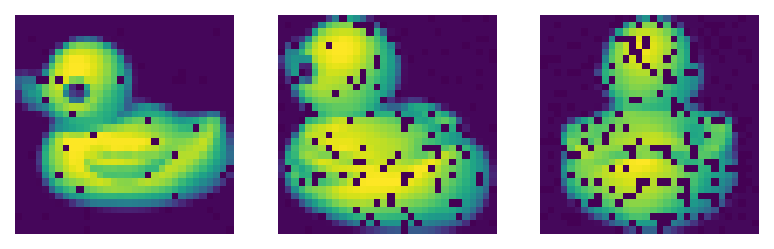
\includegraphics[width=0.32\linewidth]{figures/Linf/Linf_corr_imgs/COIL/ms_005-010-020.pdf}}}\hspace{0.001\linewidth}
\subfloat[ms-10-10-10] {\frame{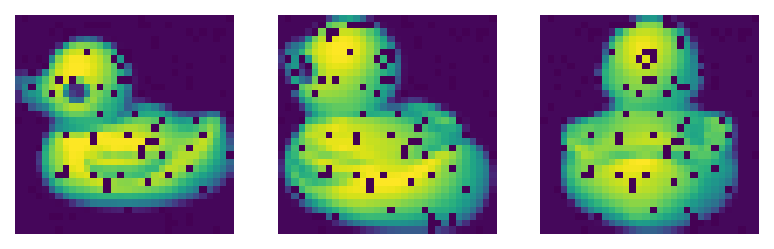
\includegraphics[width=0.32\linewidth]{figures/Linf/Linf_corr_imgs/COIL/ms_010-010-010.pdf}}}\hspace{0.001\linewidth}
\subfloat[ms-10-20-30] {\frame{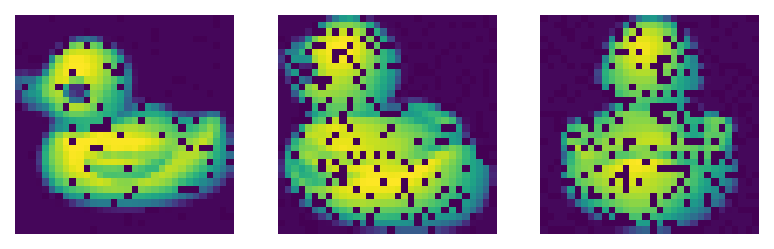
\includegraphics[width=0.32\linewidth]{figures/Linf/Linf_corr_imgs/COIL/ms_010-020-030.pdf}}}\hspace{0.001\linewidth}
\subfloat[ms-10-30-50] {\frame{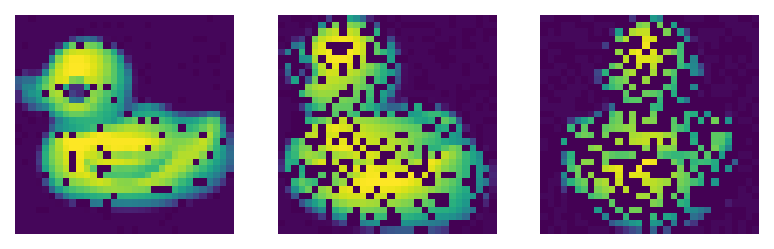
\includegraphics[width=0.32\linewidth]{figures/Linf/Linf_corr_imgs/COIL/ms_010-030-050.pdf}}}\hspace{0.001\linewidth}
\subfloat[ms-10-50-90] {\frame{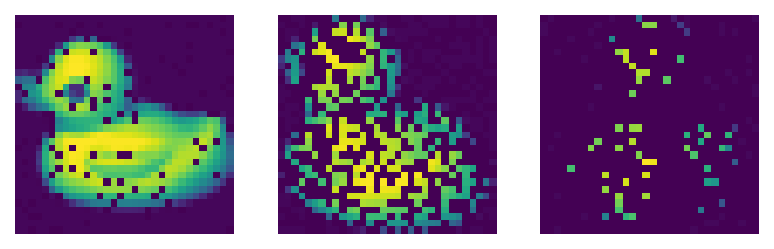
\includegraphics[width=0.32\linewidth]{figures/Linf/Linf_corr_imgs/COIL/ms_010-050-090.pdf}}}\hspace{0.001\linewidth}
\subfloat[ms-20-20-20] {\frame{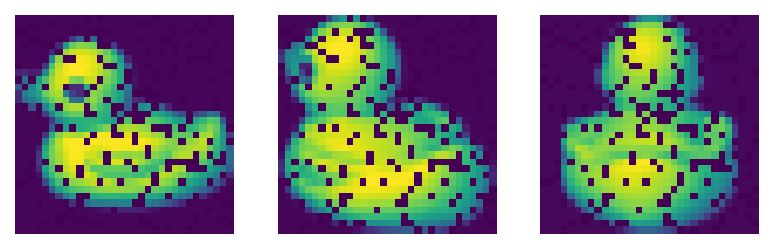
\includegraphics[width=0.32\linewidth]{figures/Linf/Linf_corr_imgs/COIL/ms_020-020-020.pdf}}}\hspace{0.001\linewidth}
\subfloat[ms-30-30-30] {\frame{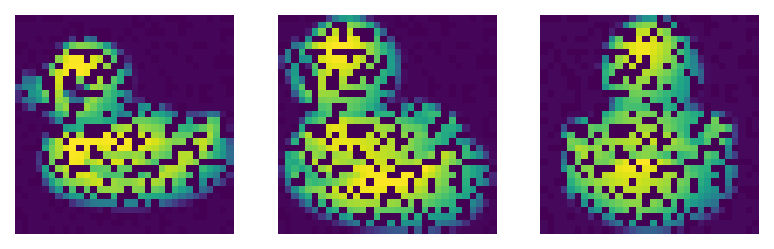
\includegraphics[width=0.32\linewidth]{figures/Linf/Linf_corr_imgs/COIL/ms_030-030-030.pdf}}}\hspace{0.001\linewidth}
\subfloat[ms-40-40-40] {\frame{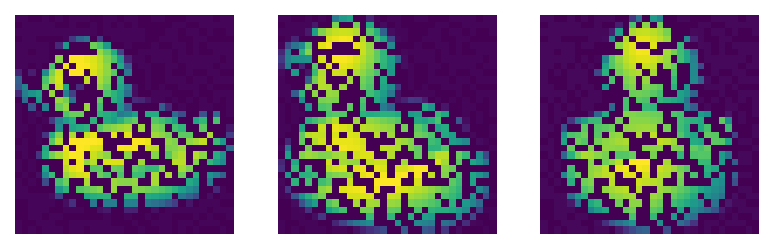
\includegraphics[width=0.32\linewidth]{figures/Linf/Linf_corr_imgs/COIL/ms_040-040-040.pdf}}}\hspace{0.001\linewidth}
\subfloat[ms-50-50-50] {\frame{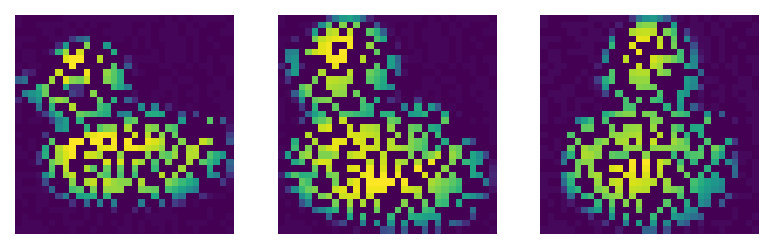
\includegraphics[width=0.32\linewidth]{figures/Linf/Linf_corr_imgs/COIL/ms_050-050-050.pdf}}}\hspace{0.001\linewidth}
\subfloat[ms-5-10-15-20] {\frame{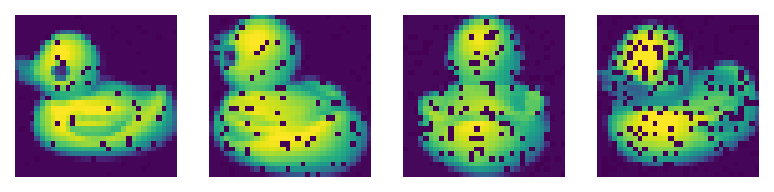
\includegraphics[width=0.32\linewidth]{figures/Linf/Linf_corr_imgs/COIL/ms_005-010-015-020.pdf}}}\hspace{0.001\linewidth}
\subfloat[ms-10-10-10-10] {\frame{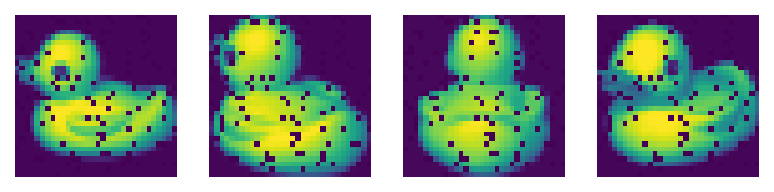
\includegraphics[width=0.32\linewidth]{figures/Linf/Linf_corr_imgs/COIL/ms_010-010-010-010.pdf}}}\hspace{0.001\linewidth}
\subfloat[ms-10-20-30-40] {\frame{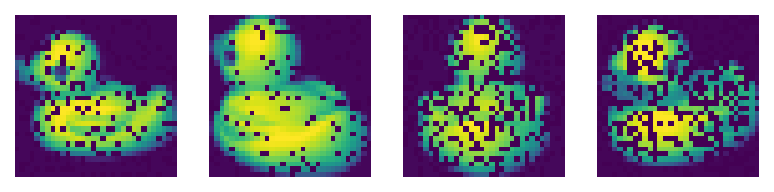
\includegraphics[width=0.32\linewidth]{figures/Linf/Linf_corr_imgs/COIL/ms_010-020-030-040.pdf}}}\hspace{0.001\linewidth}
\end{sidewaysfigure}

\begin{sidewaysfigure}[!ht]
\ContinuedFloat
\centering
\subfloat[ms-10-30-50-70] {\frame{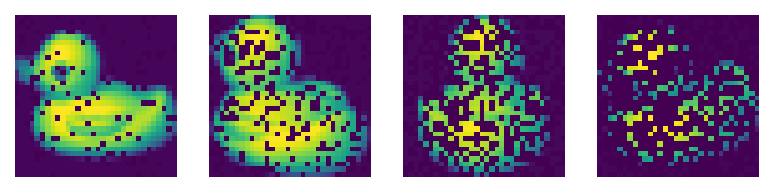
\includegraphics[width=0.32\linewidth]{figures/Linf/Linf_corr_imgs/COIL/ms_010-030-050-070.pdf}}}\hspace{0.001\linewidth}
\subfloat[ms-20-20-20-20] {\frame{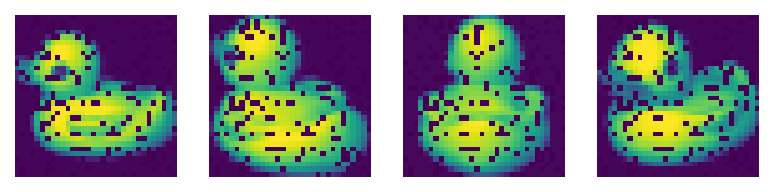
\includegraphics[width=0.32\linewidth]{figures/Linf/Linf_corr_imgs/COIL/ms_020-020-020-020.pdf}}}\hspace{0.001\linewidth}
\subfloat[ms-30-30-30-30] {\frame{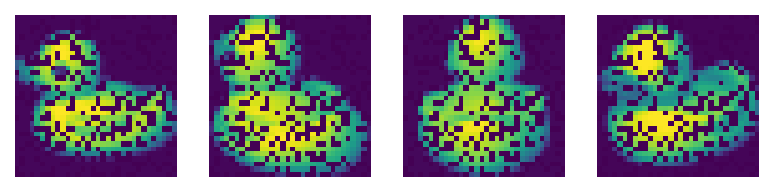
\includegraphics[width=0.32\linewidth]{figures/Linf/Linf_corr_imgs/COIL/ms_030-030-030-030.pdf}}}\hspace{0.001\linewidth}
\subfloat[ms-40-40-40-40] {\frame{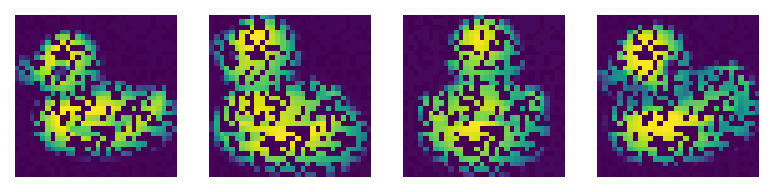
\includegraphics[width=0.32\linewidth]{figures/Linf/Linf_corr_imgs/COIL/ms_040-040-040-040.pdf}}}\hspace{0.001\linewidth}
\subfloat[ms-50-50-50-50] {\frame{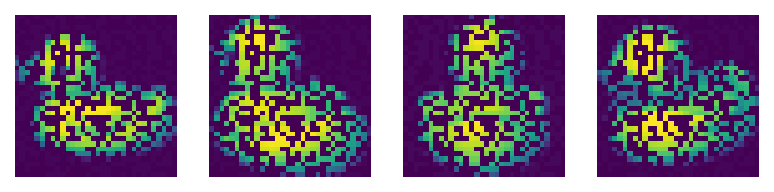
\includegraphics[width=0.32\linewidth]{figures/Linf/Linf_corr_imgs/COIL/ms_050-050-050-050.pdf}}}\hspace{0.001\linewidth}
\subfloat[sp-5-10-20] {\frame{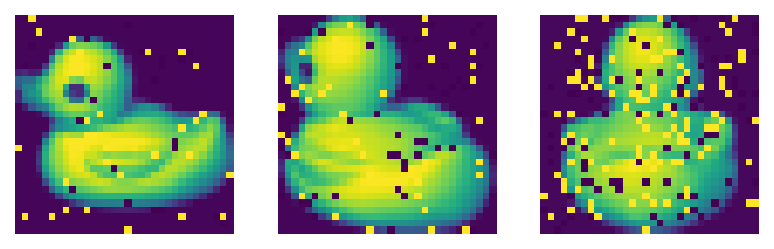
\includegraphics[width=0.32\linewidth]{figures/Linf/Linf_corr_imgs/COIL/sp_005-010-020.pdf}}}\hspace{0.001\linewidth}
\subfloat[sp-10-10-10] {\frame{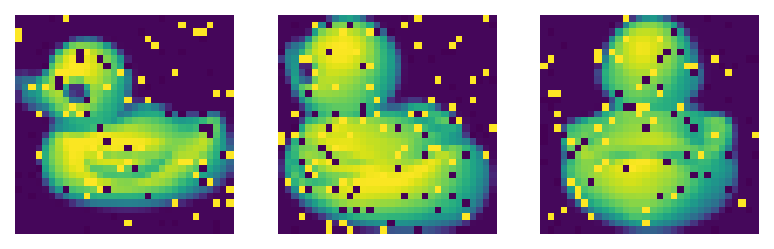
\includegraphics[width=0.32\linewidth]{figures/Linf/Linf_corr_imgs/COIL/sp_010-010-010.pdf}}}\hspace{0.001\linewidth}
\subfloat[sp-10-20-30] {\frame{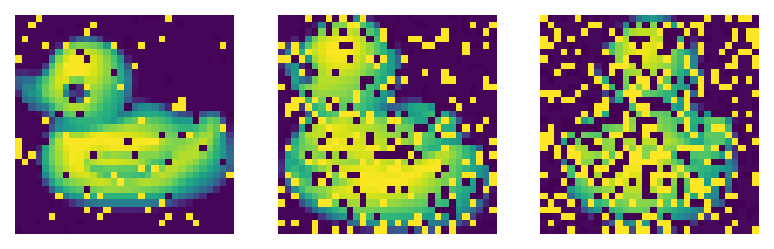
\includegraphics[width=0.32\linewidth]{figures/Linf/Linf_corr_imgs/COIL/sp_010-020-030.pdf}}}\hspace{0.001\linewidth}
\subfloat[sp-10-30-50] {\frame{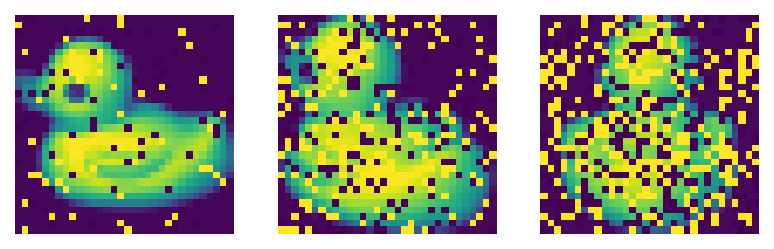
\includegraphics[width=0.32\linewidth]{figures/Linf/Linf_corr_imgs/COIL/sp_010-030-050.pdf}}}\hspace{0.001\linewidth}
\subfloat[sp-10-50-90] {\frame{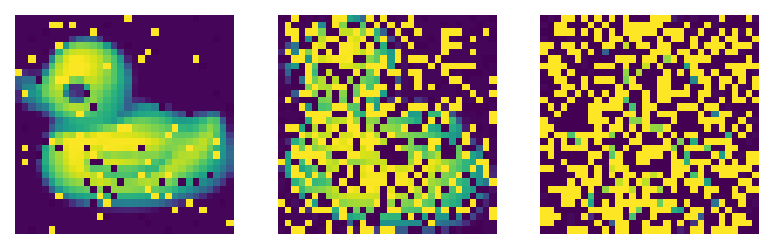
\includegraphics[width=0.32\linewidth]{figures/Linf/Linf_corr_imgs/COIL/sp_010-050-090.pdf}}}\hspace{0.001\linewidth}
\subfloat[sp-20-20-20] {\frame{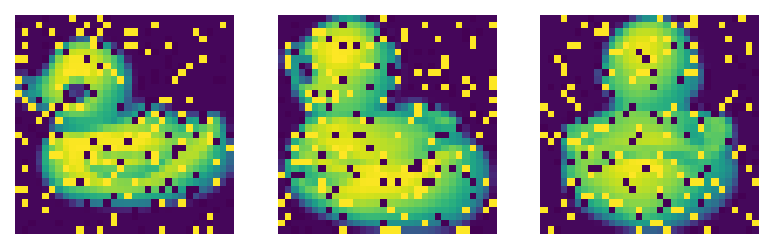
\includegraphics[width=0.32\linewidth]{figures/Linf/Linf_corr_imgs/COIL/sp_020-020-020.pdf}}}\hspace{0.001\linewidth}
\subfloat[sp-30-30-30] {\frame{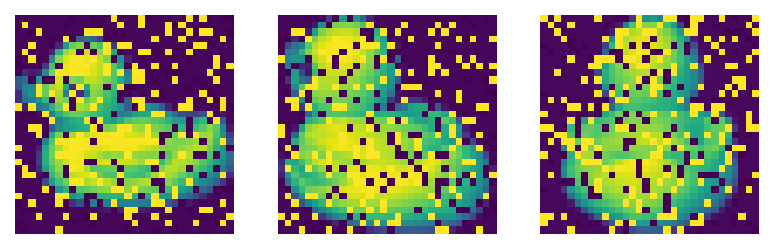
\includegraphics[width=0.32\linewidth]{figures/Linf/Linf_corr_imgs/COIL/sp_030-030-030.pdf}}}\hspace{0.001\linewidth}
\end{sidewaysfigure}

\begin{sidewaysfigure}[!ht]
\ContinuedFloat
\centering
\subfloat[sp-40-40-40] {\frame{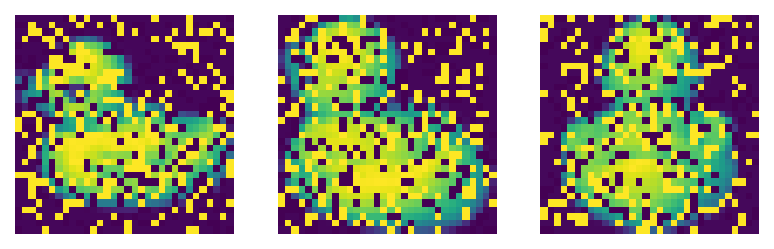
\includegraphics[width=0.32\linewidth]{figures/Linf/Linf_corr_imgs/COIL/sp_040-040-040.pdf}}}\hspace{0.001\linewidth}
\subfloat[sp-50-50-50] {\frame{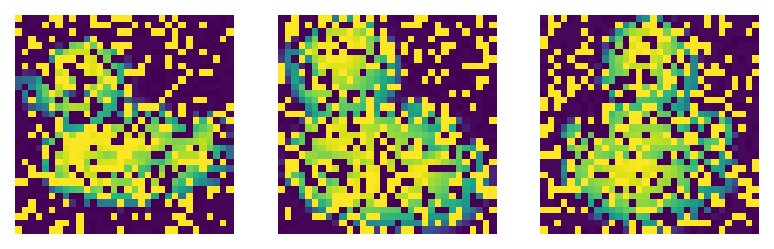
\includegraphics[width=0.32\linewidth]{figures/Linf/Linf_corr_imgs/COIL/sp_050-050-050.pdf}}}\hspace{0.001\linewidth}
\subfloat[sp-5-10-15-20] {\frame{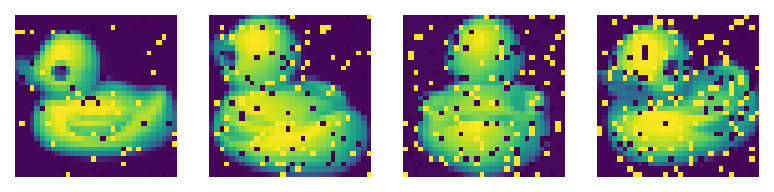
\includegraphics[width=0.32\linewidth]{figures/Linf/Linf_corr_imgs/COIL/sp_005-010-015-020.pdf}}}\hspace{0.001\linewidth}
\subfloat[sp-10-10-10-10] {\frame{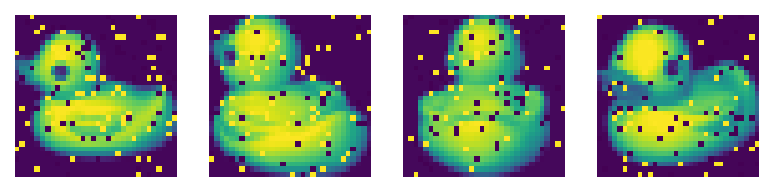
\includegraphics[width=0.32\linewidth]{figures/Linf/Linf_corr_imgs/COIL/sp_010-010-010-010.pdf}}}\hspace{0.001\linewidth}
\subfloat[sp-10-20-30-40] {\frame{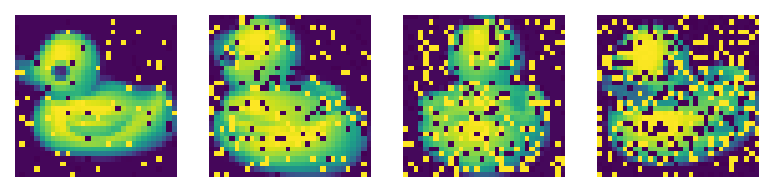
\includegraphics[width=0.32\linewidth]{figures/Linf/Linf_corr_imgs/COIL/sp_010-020-030-040.pdf}}}\hspace{0.001\linewidth}
\subfloat[sp-10-30-50-70] {\frame{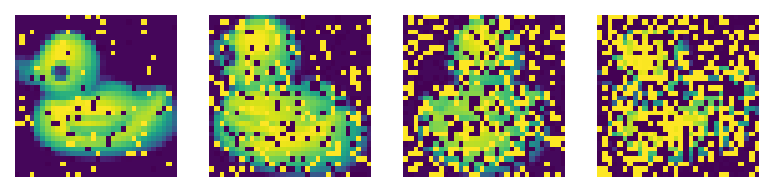
\includegraphics[width=0.32\linewidth]{figures/Linf/Linf_corr_imgs/COIL/sp_010-030-050-070.pdf}}}\hspace{0.001\linewidth}
\subfloat[sp-20-20-20-20] {\frame{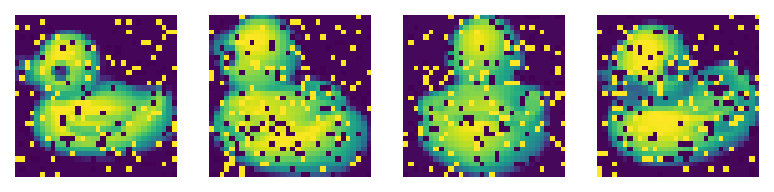
\includegraphics[width=0.32\linewidth]{figures/Linf/Linf_corr_imgs/COIL/sp_020-020-020-020.pdf}}}\hspace{0.001\linewidth}
\subfloat[sp-30-30-30-30] {\frame{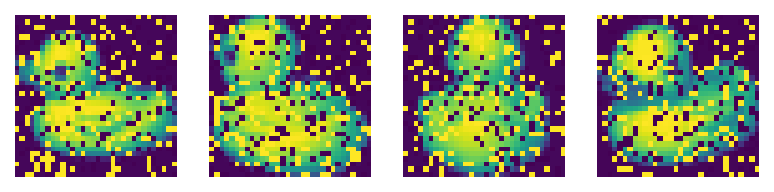
\includegraphics[width=0.32\linewidth]{figures/Linf/Linf_corr_imgs/COIL/sp_030-030-030-030.pdf}}}\hspace{0.001\linewidth}
\subfloat[sp-40-40-40-40] {\frame{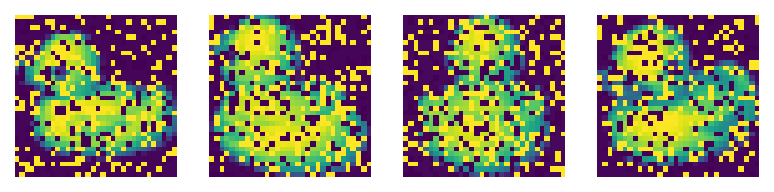
\includegraphics[width=0.32\linewidth]{figures/Linf/Linf_corr_imgs/COIL/sp_040-040-040-040.pdf}}}\hspace{0.001\linewidth}
\subfloat[sp-50-50-50-50] {\frame{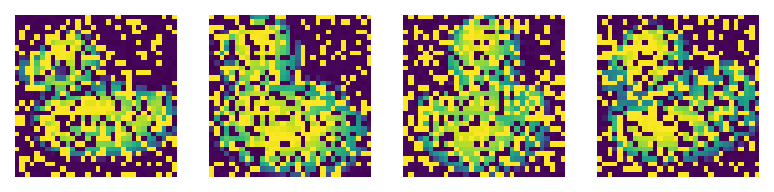
\includegraphics[width=0.32\linewidth]{figures/Linf/Linf_corr_imgs/COIL/sp_050-050-050-050.pdf}}}\hspace{0.001\linewidth}
\caption{COIL20数据集上的带噪声图像示意}
\label{fig:corr-coil}
\end{sidewaysfigure}

\begin{sidewaysfigure}[!ht]
\centering
\subfloat[ms-5-10-20] {\frame{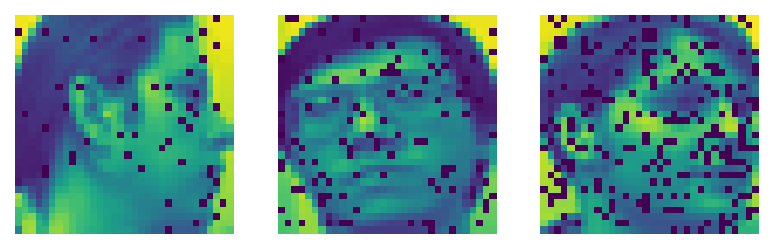
\includegraphics[width=0.32\linewidth]{figures/Linf/Linf_corr_imgs/UMIST/ms_005-010-020.pdf}}}\hspace{0.001\linewidth}
\subfloat[ms-10-10-10] {\frame{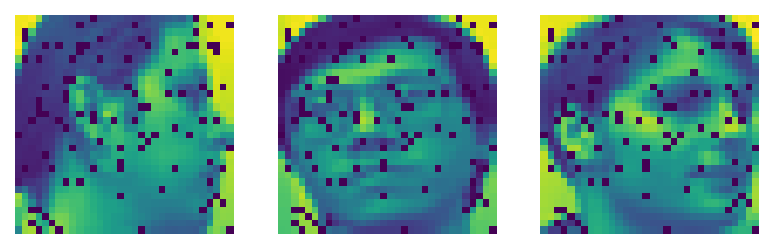
\includegraphics[width=0.32\linewidth]{figures/Linf/Linf_corr_imgs/UMIST/ms_010-010-010.pdf}}}\hspace{0.001\linewidth}
\subfloat[ms-10-20-30] {\frame{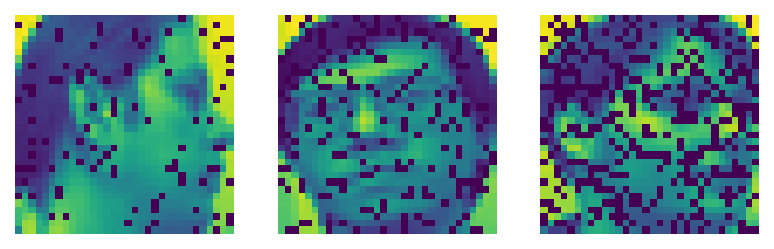
\includegraphics[width=0.32\linewidth]{figures/Linf/Linf_corr_imgs/UMIST/ms_010-020-030.pdf}}}\hspace{0.001\linewidth}
\subfloat[ms-10-30-50] {\frame{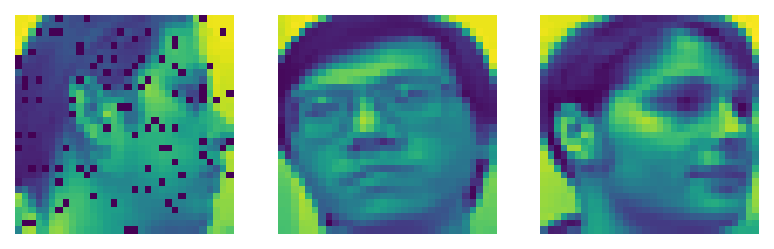
\includegraphics[width=0.32\linewidth]{figures/Linf/Linf_corr_imgs/UMIST/ms_010-030-050.pdf}}}\hspace{0.001\linewidth}
\subfloat[ms-10-50-90] {\frame{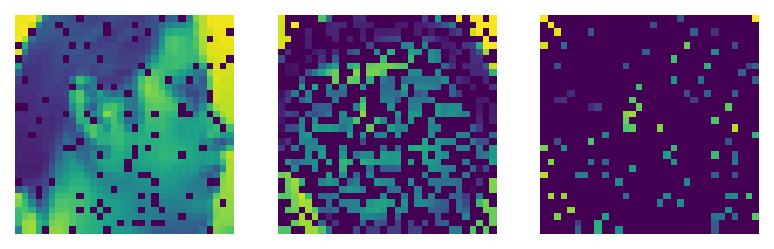
\includegraphics[width=0.32\linewidth]{figures/Linf/Linf_corr_imgs/UMIST/ms_010-050-090.pdf}}}\hspace{0.001\linewidth}
\subfloat[ms-20-20-20] {\frame{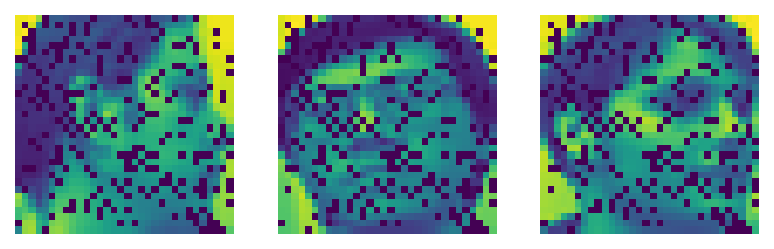
\includegraphics[width=0.32\linewidth]{figures/Linf/Linf_corr_imgs/UMIST/ms_020-020-020.pdf}}}\hspace{0.001\linewidth}
\subfloat[ms-30-30-30] {\frame{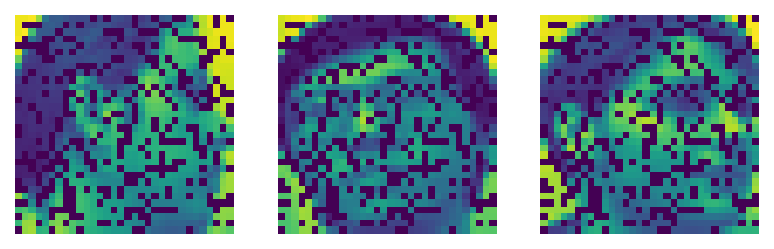
\includegraphics[width=0.32\linewidth]{figures/Linf/Linf_corr_imgs/UMIST/ms_030-030-030.pdf}}}\hspace{0.001\linewidth}
\subfloat[ms-40-40-40] {\frame{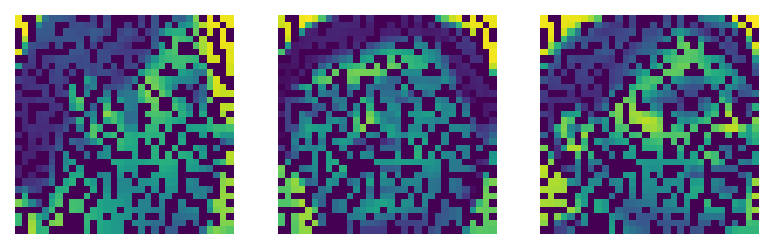
\includegraphics[width=0.32\linewidth]{figures/Linf/Linf_corr_imgs/UMIST/ms_040-040-040.pdf}}}\hspace{0.001\linewidth}
\subfloat[ms-50-50-50] {\frame{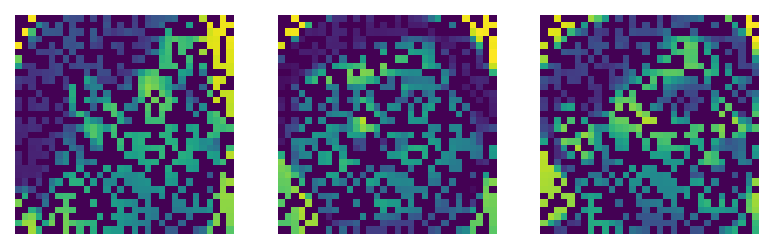
\includegraphics[width=0.32\linewidth]{figures/Linf/Linf_corr_imgs/UMIST/ms_050-050-050.pdf}}}\hspace{0.001\linewidth}
\subfloat[sp-5-10-20] {\frame{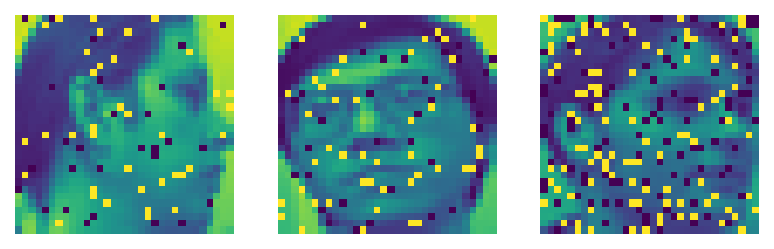
\includegraphics[width=0.32\linewidth]{figures/Linf/Linf_corr_imgs/UMIST/sp_005-010-020.pdf}}}\hspace{0.001\linewidth}
\subfloat[sp-10-10-10] {\frame{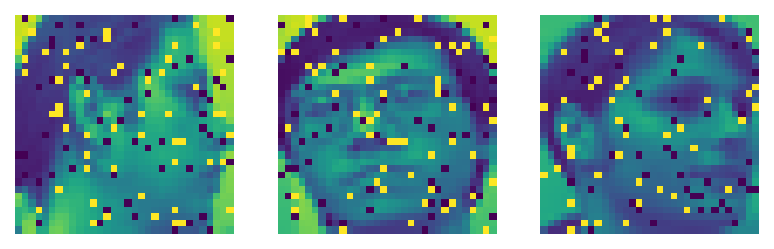
\includegraphics[width=0.32\linewidth]{figures/Linf/Linf_corr_imgs/UMIST/sp_010-010-010.pdf}}}\hspace{0.001\linewidth}
\subfloat[sp-10-20-30] {\frame{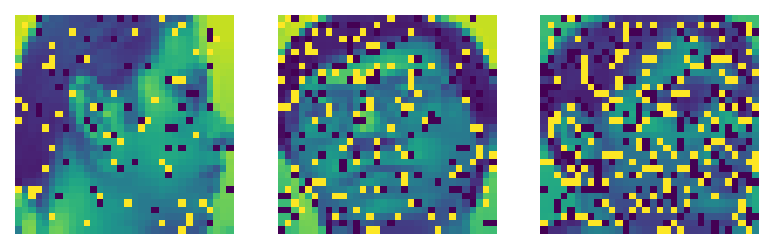
\includegraphics[width=0.32\linewidth]{figures/Linf/Linf_corr_imgs/UMIST/sp_010-020-030.pdf}}}\hspace{0.001\linewidth}
\end{sidewaysfigure}

\begin{sidewaysfigure}[!ht]
\ContinuedFloat
\centering
\subfloat[sp-10-30-50] {\frame{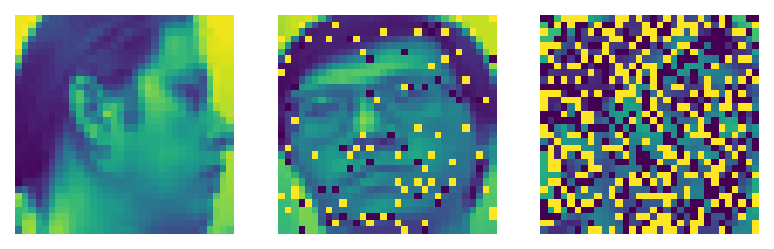
\includegraphics[width=0.32\linewidth]{figures/Linf/Linf_corr_imgs/UMIST/sp_010-030-050.pdf}}}\hspace{0.001\linewidth}
\subfloat[sp-10-50-90] {\frame{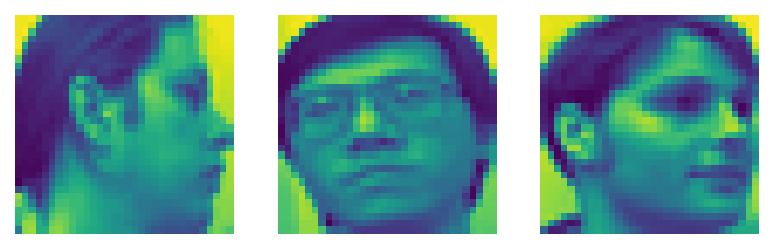
\includegraphics[width=0.32\linewidth]{figures/Linf/Linf_corr_imgs/UMIST/sp_010-050-090.pdf}}}\hspace{0.001\linewidth}
\subfloat[ms-20-20-20] {\frame{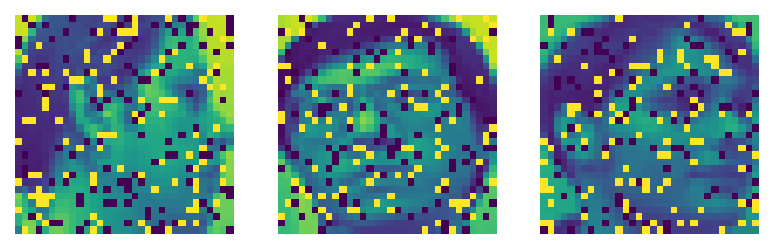
\includegraphics[width=0.32\linewidth]{figures/Linf/Linf_corr_imgs/UMIST/sp_020-020-020.pdf}}}\hspace{0.001\linewidth}
\subfloat[sp-30-30-30] {\frame{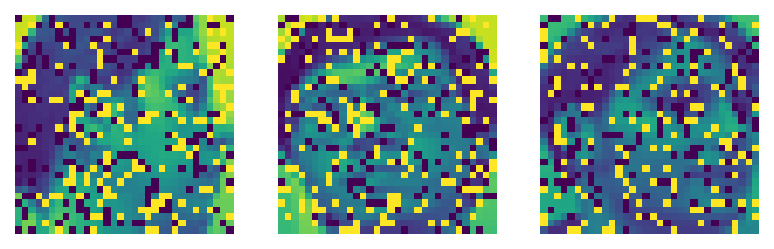
\includegraphics[width=0.32\linewidth]{figures/Linf/Linf_corr_imgs/UMIST/sp_030-030-030.pdf}}}\hspace{0.001\linewidth}
\subfloat[sp-40-40-40] {\frame{\includegraphics[width=0.32\linewidth]{figures/Linf/Linf_corr_imgs/UMIST/sp_040-040-040.pdf}}}\hspace{0.001\linewidth}
\subfloat[sp-50-50-50] {\frame{\includegraphics[width=0.32\linewidth]{figures/Linf/Linf_corr_imgs/UMIST/sp_050-050-050.pdf}}}\hspace{0.001\linewidth}
\caption{UMIST数据集上的带噪声图像示意}
\label{fig:corr-umist}
\subfloat[ms-5-10-20] {\frame{\includegraphics[width=0.32\linewidth]{figures/Linf/Linf_corr_imgs/YALE/ms_005-010-020.pdf}}}\hspace{0.001\linewidth}
\subfloat[ms-10-10-10] {\frame{\includegraphics[width=0.32\linewidth]{figures/Linf/Linf_corr_imgs/YALE/ms_010-010-010.pdf}}}\hspace{0.001\linewidth}
\subfloat[ms-10-20-30] {\frame{\includegraphics[width=0.32\linewidth]{figures/Linf/Linf_corr_imgs/YALE/ms_010-020-030.pdf}}}\hspace{0.001\linewidth}
\subfloat[ms-10-30-50] {\frame{\includegraphics[width=0.32\linewidth]{figures/Linf/Linf_corr_imgs/YALE/ms_010-030-050.pdf}}}\hspace{0.001\linewidth}
\subfloat[ms-10-50-90] {\frame{\includegraphics[width=0.32\linewidth]{figures/Linf/Linf_corr_imgs/YALE/ms_010-050-090.pdf}}}\hspace{0.001\linewidth}
\subfloat[ms-20-20-20] {\frame{\includegraphics[width=0.32\linewidth]{figures/Linf/Linf_corr_imgs/YALE/ms_020-020-020.pdf}}}\hspace{0.001\linewidth}
\end{sidewaysfigure}

% \begin{sidewaysfigure}[!ht]
% \centering
% \subfloat[ms-5-10-20] {\frame{\includegraphics[width=0.32\linewidth]{figures/Linf/Linf_corr_imgs/YALE/ms_005-010-020.pdf}}}\hspace{0.001\linewidth}
% \subfloat[ms-10-10-10] {\frame{\includegraphics[width=0.32\linewidth]{figures/Linf/Linf_corr_imgs/YALE/ms_010-010-010.pdf}}}\hspace{0.001\linewidth}
% \subfloat[ms-10-20-30] {\frame{\includegraphics[width=0.32\linewidth]{figures/Linf/Linf_corr_imgs/YALE/ms_010-020-030.pdf}}}\hspace{0.001\linewidth}
% \subfloat[ms-10-30-50] {\frame{\includegraphics[width=0.32\linewidth]{figures/Linf/Linf_corr_imgs/YALE/ms_010-030-050.pdf}}}\hspace{0.001\linewidth}
% \subfloat[ms-10-50-90] {\frame{\includegraphics[width=0.32\linewidth]{figures/Linf/Linf_corr_imgs/YALE/ms_010-050-090.pdf}}}\hspace{0.001\linewidth}
% \subfloat[ms-20-20-20] {\frame{\includegraphics[width=0.32\linewidth]{figures/Linf/Linf_corr_imgs/YALE/ms_020-020-020.pdf}}}\hspace{0.001\linewidth}
% \end{sidewaysfigure}

\begin{sidewaysfigure}[!ht]
\ContinuedFloat
\centering
\subfloat[ms-30-30-30] {\frame{\includegraphics[width=0.32\linewidth]{figures/Linf/Linf_corr_imgs/YALE/ms_030-030-030.pdf}}}\hspace{0.001\linewidth}
\subfloat[ms-40-40-40] {\frame{\includegraphics[width=0.32\linewidth]{figures/Linf/Linf_corr_imgs/YALE/ms_040-040-040.pdf}}}\hspace{0.001\linewidth}
\subfloat[ms-50-50-50] {\frame{\includegraphics[width=0.32\linewidth]{figures/Linf/Linf_corr_imgs/YALE/ms_050-050-050.pdf}}}\hspace{0.001\linewidth}
\subfloat[sp-5-10-20] {\frame{\includegraphics[width=0.32\linewidth]{figures/Linf/Linf_corr_imgs/YALE/sp_005-010-020.pdf}}}\hspace{0.001\linewidth}
\subfloat[sp-10-10-10] {\frame{\includegraphics[width=0.32\linewidth]{figures/Linf/Linf_corr_imgs/YALE/sp_010-010-010.pdf}}}\hspace{0.001\linewidth}
\subfloat[sp-10-20-30] {\frame{\includegraphics[width=0.32\linewidth]{figures/Linf/Linf_corr_imgs/YALE/sp_010-020-030.pdf}}}\hspace{0.001\linewidth}
\subfloat[sp-10-30-50] {\frame{\includegraphics[width=0.32\linewidth]{figures/Linf/Linf_corr_imgs/YALE/sp_010-030-050.pdf}}}\hspace{0.001\linewidth}
\subfloat[sp-10-50-90] {\frame{\includegraphics[width=0.32\linewidth]{figures/Linf/Linf_corr_imgs/YALE/sp_010-050-090.pdf}}}\hspace{0.001\linewidth}
\subfloat[sp-20-20-20] {\frame{\includegraphics[width=0.32\linewidth]{figures/Linf/Linf_corr_imgs/YALE/sp_020-020-020.pdf}}}\hspace{0.001\linewidth}
\subfloat[sp-30-30-30] {\frame{\includegraphics[width=0.32\linewidth]{figures/Linf/Linf_corr_imgs/YALE/sp_030-030-030.pdf}}}\hspace{0.001\linewidth}
\subfloat[sp-40-40-40] {\frame{\includegraphics[width=0.32\linewidth]{figures/Linf/Linf_corr_imgs/YALE/sp_040-040-040.pdf}}}\hspace{0.001\linewidth}
\subfloat[sp-50-50-50] {\frame{\includegraphics[width=0.32\linewidth]{figures/Linf/Linf_corr_imgs/YALE/sp_050-050-050.pdf}}}\hspace{0.001\linewidth}
\caption{Yale数据集上的带噪声图像示意}
\label{fig:corr-yale}
\end{sidewaysfigure}
    

\end{apdix}